% Lưu ý: Đảm bảo đã thêm \usepackage{booktabs} và \usepackage{subcaption} vào main.tex
% Lưu ý: Cần chuẩn bị các file ảnh từ PDF và thêm các môi trường \begin{figure}...\end{figure} tương ứng.
\chapter{KIẾN TRÚC HỆ THỐNG VÀ LÝ THUYẾT CƠ SỞ} % Revised Title
\label{Chapter2}
Chương \ref{Chapter2} trình bày các khái niệm lý thuyết cơ bản liên quan đến hệ thống được triển khai trong báo cáo này, bao gồm Hệ thống trên Chip (\acrshort{soc}), bộ xử lý mềm Nios V, Truy cập Bộ nhớ Trực tiếp (\acrshort{dma}), chuẩn giao tiếp Avalon, và cuối cùng là thiết kế và kiến trúc cụ thể của bộ điều khiển DMA tùy chỉnh được sử dụng.

\section{Tổng quan về Hệ thống trên Chip (SoC)}
\acrfull{soc} là một vi mạch (\acrshort{ic}) tích hợp hầu hết hoặc tất cả các thành phần của một máy tính hoặc hệ thống điện tử khác vào một chip duy nhất. Nó có thể chứa các thành phần kỹ thuật số, tương tự, tín hiệu hỗn hợp và thường cả tần số vô tuyến - tất cả trên một đế chip. Một \acrshort{soc} điển hình bao gồm:
\begin{itemize}
    \item Một hoặc nhiều lõi vi xử lý (Microprocessor cores) hoặc vi điều khiển (Microcontroller cores).
    \item Các khối bộ nhớ như \acrshort{ram}, \acrshort{rom}, EEPROM hoặc Flash.
    \item Các bộ định thời (Timers), bộ đếm (Counters).
    \item Các giao tiếp ngoại vi như \acrshort{uart}, SPI, I2C, \acrshort{usb}.
    \item Các khối xử lý tín hiệu số (\acrshort{dsp}).
    \item Các bộ chuyển đổi tương tự-số (ADC) và số-tương tự (DAC).
    \item Hệ thống kết nối nội bộ (interconnect) như bus (ví dụ: AMBA AXI, Avalon).
\end{itemize}
Trong bối cảnh \acrshort{fpga}, \acrshort{soc} thường đề cập đến việc tích hợp một hoặc nhiều lõi xử lý mềm (soft-core) hoặc cứng (hard-core) cùng với các ngoại vi và bộ nhớ trên cùng một cấu trúc \acrshort{fpga}, sử dụng các công cụ như Intel Platform Designer.

\section{Bộ xử lý mềm Intel Nios V/m}
Nios V là thế hệ bộ xử lý mềm (soft-core processor) mới nhất của Intel dựa trên kiến trúc tập lệnh (ISA) RISC-V mã nguồn mở \cite{intelNiosVHandbook}. Là một bộ xử lý mềm, Nios V được triển khai hoàn toàn bằng logic \acrshort{fpga}, mang lại sự linh hoạt cao trong việc cấu hình và tích hợp vào các thiết kế \acrshort{soc}.
\begin{itemize}
    \item \textbf{Nios V/m (Microcontroller):} Phiên bản được sử dụng trong báo cáo này là \acrshort{niosv}/m (RV32IMAZicsr), được tối ưu hóa cho các ứng dụng vi điều khiển, nhấn mạnh vào diện tích logic nhỏ và hiệu quả năng lượng. Nó phù hợp cho các nhiệm vụ điều khiển, quản lý ngoại vi và xử lý cơ bản trong hệ thống nhúng, đáp ứng nhu cầu của một bộ vi xử lý cơ bản.
    \item \textbf{Kiến trúc RISC-V:} Dựa trên ISA RISC-V mã nguồn mở, cung cấp một kiến trúc hiện đại, module hóa và không ràng buộc về bản quyền. Nios V/m triển khai tập lệnh cơ sở RV32I cùng với các mở rộng tiêu chuẩn như M (Integer Multiplication and Division), A (Atomic Instructions), Zicsr (Control and Status Register Access).
    \begin{figure}[htbp]
        \centering
        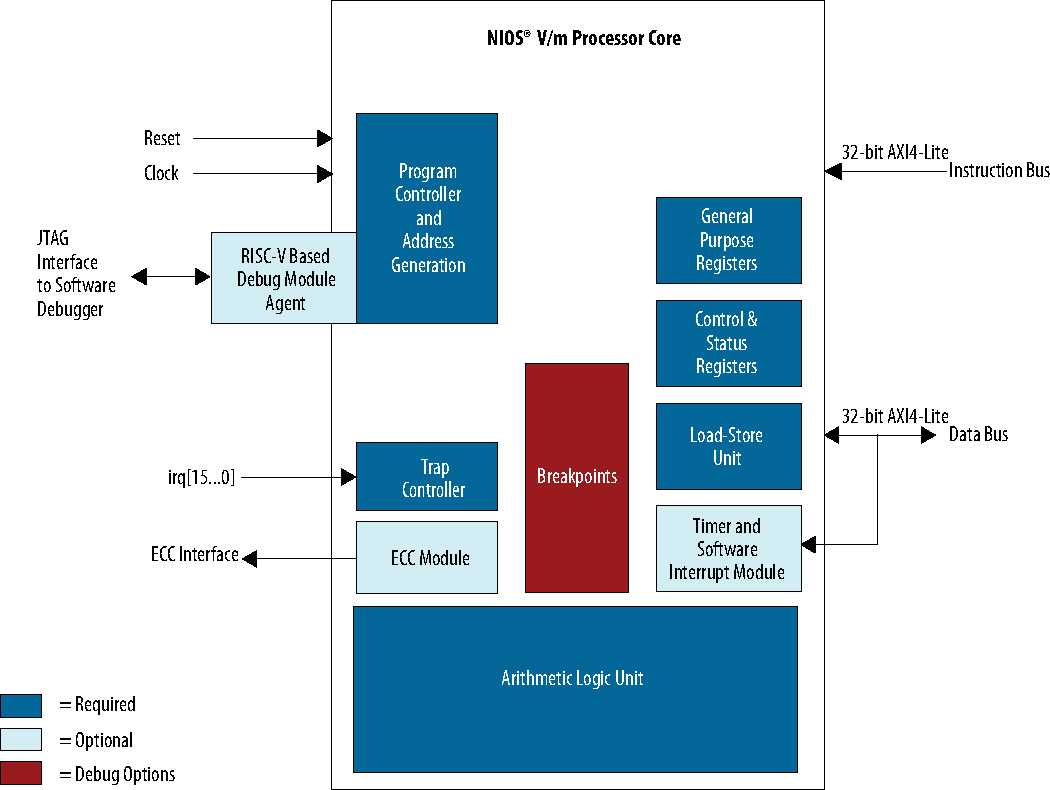
\includegraphics[width=0.6\linewidth]{Images/02_00_NiosVm_Architecture.pdf}
        \caption{Kiến trúc Nios V/m \cite{niosv_architecture}.}
        \label{fig:niosv_architecture}
    \end{figure}
    \item \textbf{Pipeline (Tùy chọn):} Nios V/m có thể được cấu hình với pipeline 5 tầng kinh điển (Fetch, Decode, Execute, Memory, Write back) để tăng hiệu suất hoặc không có pipeline (non-pipelined) để tối ưu diện tích. Khi sử dụng pipeline, có thể xảy ra hiện tượng stall (trì hoãn) do phụ thuộc dữ liệu (data dependency) hoặc tranh chấp tài nguyên (resource stall).
\end{itemize}

\section{Truy cập Bộ nhớ Trực tiếp (DMA)}
\acrfull{dma} là một tính năng của hệ thống máy tính cho phép một số hệ thống con phần cứng nhất định truy cập bộ nhớ hệ thống chính (\acrshort{ram}) để đọc và/hoặc ghi một cách độc lập với bộ xử lý trung tâm (CPU).
\begin{itemize}
    \item \textbf{Mục đích:} Giảm tải cho CPU trong các tác vụ truyền dữ liệu khối lượng lớn giữa bộ nhớ và các thiết bị ngoại vi (hoặc giữa các vùng nhớ khác nhau). Khi CPU khởi tạo một hoạt động DMA, nó có thể thực hiện các công việc khác trong khi bộ điều khiển DMA (DMA Controller - DMAC) thực hiện việc truyền dữ liệu.
    \item \textbf{Hoạt động:} CPU cấu hình DMAC với địa chỉ nguồn, địa chỉ đích, và số lượng dữ liệu cần truyền. Sau đó, CPU ra lệnh cho DMAC bắt đầu. DMAC chiếm quyền điều khiển bus hệ thống (hoặc sử dụng một bus riêng) để thực hiện việc truyền dữ liệu trực tiếp. Khi hoàn tất, DMAC thường thông báo cho CPU thông qua một ngắt (interrupt) hoặc bằng cách đặt một cờ trạng thái.
    \item \textbf{Lợi ích:} Tăng thông lượng dữ liệu, giải phóng CPU cho các tác vụ tính toán khác, cải thiện hiệu suất hệ thống tổng thể, đặc biệt quan trọng trong các hệ thống xử lý dữ liệu lớn hoặc thời gian thực.
\end{itemize}

% --- Section 4: Avalon Bus (Đã di chuyển từ Section 6 cũ) ---
\section{Giao tiếp Hệ thống: Bus Avalon}
\label{sec:avalon_bus}
Trong các hệ thống SoC được thiết kế trên nền tảng FPGA của Intel bằng công cụ Platform Designer, Giao tiếp Bus Avalon đóng vai trò là chuẩn kết nối (interconnect) nền tảng. 

Đặc tả Avalon bao gồm nhiều loại giao diện con, trong đó Avalon Memory-Mapped (Avalon-MM) là giao diện được sử dụng chủ yếu trong thiết kế bộ điều khiển DMA này để truy cập bộ nhớ và thanh ghi điều khiển.

\subsection{Giao tiếp Bus Avalon Memory Mapped Interface (Avalon-MM)}
Avalon-MM là một giao diện dựa trên địa chỉ, được thiết kế theo kiến trúc Master-Slave cho các giao dịch truy cập vào không gian bộ nhớ hoặc thanh ghi.

% Figure 02_01 (Existing)
\begin{figure}[htbp]
    \centering
    % Assumes this PDF is in the Images folder
    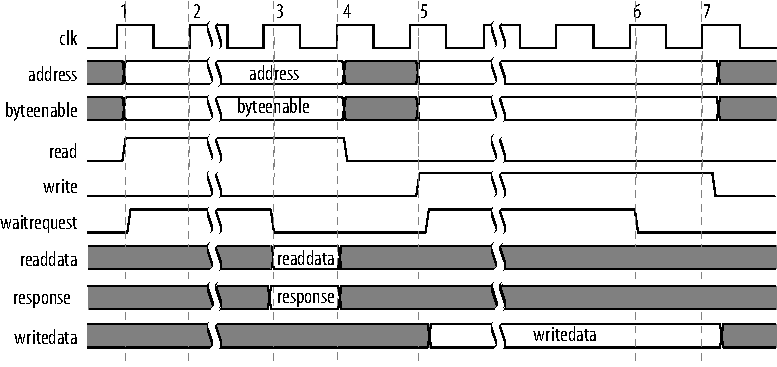
\includegraphics[width=\linewidth]{Images/02_01_Avalon_MM_Transfers.pdf}
    \caption{Các giao dịch đọc và ghi Avalon-MM điển hình với tín hiệu waitrequest \cite{avalon_mm_transfer}.}
    \label{fig:02_01_avalon_mm_transfer} % Kept original label
\end{figure}

\subsubsection{Đặc tả và Yêu cầu Giao thức}
\begin{itemize}
    \item \textbf{Vai trò Master/Slave:} 
    \begin{itemize}
        \item Một giao dịch luôn được khởi tạo bởi Master (ví dụ: CPU, DMA Master) và được phản hồi bởi Slave (ví dụ: Bộ nhớ, Thanh ghi DMA).
        \item Master chịu trách nhiệm cung cấp địa chỉ và tín hiệu điều khiển (\texttt{read}, \texttt{write}, \texttt{byteenable}), trong khi Slave giải mã địa chỉ, phản hồi bằng dữ liệu (\texttt{readdata}) hoặc chấp nhận ghi dữ liệu (\texttt{writedata}), và có thể sử dụng tín hiệu điều khiển luồng (\texttt{waitrequest}, \texttt{readdatavalid}).
    \end{itemize} 
    \item \textbf{Giao dịch Đọc (Read Transaction):}
        \begin{itemize}
            \item Master kích hoạt tín hiệu \texttt{read=1} và đưa ra \texttt{address}.
            \item Slave, sau khi giải mã địa chỉ và sẵn sàng dữ liệu, sẽ đặt dữ liệu lên \texttt{readdata}.
            \item \textbf{Điều khiển luồng (\texttt{waitrequest}):} Nếu Slave cần thêm thời gian (ví dụ: bộ nhớ chậm), nó sẽ kích hoạt \texttt{waitrequest=1}. Master \textit{phải} giữ nguyên \texttt{address} và \texttt{read} cho đến khi \texttt{waitrequest} bị hủy kích hoạt (\texttt{=0}). Slave trả về \texttt{readdata} trong chu kỳ clock mà \texttt{read=1} và \texttt{waitrequest=0}.
            \item \textbf{Tính hợp lệ dữ liệu (\texttt{readdatavalid}):} Trong các giao dịch đọc có độ trễ thay đổi (variable-latency reads, thường là pipelined), Slave sẽ kích hoạt \texttt{readdatavalid=1} cùng lúc với \texttt{readdata} để báo hiệu dữ liệu hợp lệ. Master \textit{phải} chỉ lấy dữ liệu khi \texttt{readdatavalid=1} (và \texttt{waitrequest=0}). Giao diện Read Master của DMA này (\texttt{READ\_MASTER}) được thiết kế để hỗ trợ \texttt{readdatavalid}.
            \item Giản đồ sóng đọc điển hình được minh họa trong Hình \ref{fig:02_01_avalon_mm_transfer} (phần Read), Hình \ref{fig:avalon_slave_waveforms}(a), \ref{fig:02_05_avalon_master_read}, và \ref{fig:memory_waveforms}(a).
        \end{itemize}
    \item \textbf{Giao dịch Ghi (Write Transaction):}
        \begin{itemize}
            \item Master kích hoạt \texttt{write=1}, đưa ra \texttt{address}, \texttt{writedata}, và \texttt{byteenable} (nếu có).
            \item \textbf{Điều khiển luồng (\texttt{waitrequest}):} Nếu Slave cần thêm thời gian để chuẩn bị nhận dữ liệu, nó sẽ kích hoạt \texttt{waitrequest=1}. Master *phải* giữ nguyên tất cả tín hiệu (\texttt{address}, \texttt{write}, \texttt{writedata}, \texttt{byteenable}) cho đến khi \texttt{waitrequest} bị hủy kích hoạt (\texttt{=0}). Slave sẽ ghi dữ liệu vào chu kỳ clock mà \texttt{write=1} và \texttt{waitrequest=0}.
            \item Tín hiệu \texttt{byteenable} cho phép ghi vào các byte cụ thể trong word dữ liệu (ví dụ: \texttt{4'b0011} chỉ ghi 2 byte thấp). Thiết kế DMA này sử dụng \texttt{byteenable=4'b1111} để ghi toàn bộ word 32-bit (Hình \ref{fig:02_02_memory_byteenable}).
            \item Giản đồ sóng ghi điển hình được minh họa trong Hình \ref{fig:02_01_avalon_mm_transfer} (phần Write), Hình \ref{fig:avalon_slave_waveforms}(b), \ref{fig:02_06_avalon_master_write}, và \ref{fig:memory_waveforms}(b).
        \end{itemize}
\end{itemize}

% Figure 02_02 (Existing, fixed label)
\begin{figure}[htbp]
    \centering
    % Assumes this PDF is in the Images folder
    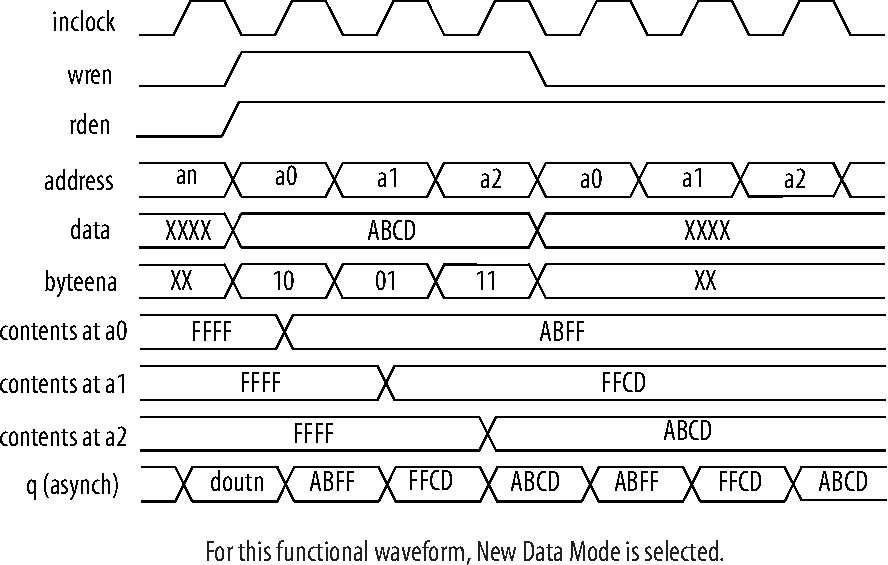
\includegraphics[width=\linewidth]{Images/02_02_Memory_ByteEnable.pdf}
    \caption{Giản đồ sóng chức năng của Byte Enable. Hình này minh họa ảnh hưởng của byte enable lên dữ liệu được ghi vào và đọc ra từ bộ nhớ \cite{memory_byteenable}.}
    \label{fig:02_02_memory_byteenable} % Fixed duplicate label
\end{figure}

Việc hiểu rõ và tuân thủ các yêu cầu về thời gian và hành vi của các tín hiệu này là cực kỳ quan trọng khi thiết kế một thành phần IP tương thích Avalon-MM.

% --- Section 5: Thiết kế và Kiến trúc DMA (Gộp từ Section 4, 5 cũ) ---
\section{Thiết kế và Kiến trúc Bộ điều khiển DMA Tùy chỉnh}
\label{sec:dma_design_and_architecture} % Label mới cho section gộp
Mục tiêu chính của việc thiết kế bộ điều khiển DMA này là tạo ra một thành phần phần cứng có khả năng truyền dữ liệu hiệu quả giữa các vùng nhớ trong hệ thống SoC trên FPGA, qua đó giảm tải cho bộ xử lý trung tâm Nios V/m. Để đạt được mục tiêu này, việc thiết kế phải tuân thủ các đặc tả giao tiếp của hệ thống bus Avalon-MM đã được trình bày ở Mục \ref{sec:avalon_bus}, đồng thời đảm bảo tính đúng đắn và hiệu quả của quá trình truyền dữ liệu.

Dựa trên yêu cầu về khả năng truyền dữ liệu tốc độ cao và độc lập với CPU, cũng như đặc tả của bus Avalon-MM, bộ điều khiển DMA tùy chỉnh được thiết kế với kiến trúc và các lựa chọn sau:

\subsection{Mục tiêu và Bối cảnh: Truyền dữ liệu giữa Bộ nhớ On-Chip}
\label{subsec:dma_context_onchip}
Một trong những ứng dụng ban đầu và quan trọng thúc đẩy việc thiết kế bộ điều khiển DMA này là nhu cầu truyền dữ liệu nhanh chóng và hiệu quả giữa các khối bộ nhớ trong chip (On-chip Memory - OCM) trên FPGA. Bộ nhớ on-chip, thường được hiện thực hóa bằng các khối RAM tích hợp sẵn trong cấu trúc FPGA, cung cấp tốc độ truy cập rất cao so với bộ nhớ ngoài (off-chip). Việc sử dụng DMA để di chuyển dữ liệu giữa các khối OCM (ví dụ: từ một vùng RAM chứa dữ liệu thô sang một vùng RAM khác để xử lý) giúp giải phóng CPU Nios V/m khỏi các vòng lặp sao chép bộ nhớ (\texttt{memcpy}) tốn thời gian, cho phép CPU tập trung vào các nhiệm vụ tính toán hoặc điều khiển khác.

Do đó, các giao diện Avalon-MM Master của \texttt{READ\_MASTER} và \texttt{WRITE\_MASTER} được thiết kế với giả định ban đầu là tương tác với các Slave là bộ nhớ on-chip. Điều này có nghĩa là chúng được tối ưu cho các giao dịch truy cập bộ nhớ có độ trễ tương đối thấp và ổn định, như được minh họa trong các giản đồ sóng đọc/ghi bộ nhớ (Hình \ref{fig:memory_waveforms}). Mặc dù vậy, thiết kế vẫn tuân thủ đầy đủ đặc tả Avalon-MM, cho phép DMA hoạt động với các loại bộ nhớ hoặc ngoại vi khác có hành vi thời gian khác nhau, miễn là chúng cũng tuân thủ chuẩn Avalon-MM.

\subsection{Kiến trúc Tổng thể và Luồng Dữ liệu}
Kiến trúc DMA được chọn dựa trên mô hình tách biệt luồng đọc và ghi dữ liệu để tối đa hóa thông lượng, bao gồm các khối chính sau:
\begin{itemize}
    \item \textbf{CONTROL\_SLAVE (`CONTROL\_SLAVE.v`):} Hoạt động như giao diện điều khiển Avalon-MM Slave cho CPU.
    \item \textbf{READ\_MASTER (`READ\_MASTER.v`):} Hoạt động như Avalon-MM Master để đọc dữ liệu từ bộ nhớ nguồn.
    \item \textbf{WRITE\_MASTER (`WRITE\_MASTER.v`):} Hoạt động như Avalon-MM Master để ghi dữ liệu vào bộ nhớ đích.
    \item \textbf{FIFO (`FIFO\_IP.v`):} Bộ đệm dữ liệu giữa Read và Write Master, được tạo từ IP Catalog của Quartus.
\end{itemize}
Luồng dữ liệu cơ bản diễn ra như sau: CPU cấu hình DMA thông qua \texttt{CONTROL\_SLAVE} (ghi địa chỉ nguồn, đích, độ dài). CPU kích hoạt DMA bằng cách ghi vào thanh ghi điều khiển. Khi được kích hoạt (\texttt{Start=1}), \texttt{READ\_MASTER} bắt đầu đọc dữ liệu từ bộ nhớ nguồn theo địa chỉ và độ dài đã cấu hình, đẩy dữ liệu vào FIFO. Đồng thời, \texttt{WRITE\_MASTER} đọc dữ liệu từ FIFO (khi FIFO không rỗng - \texttt{FF\_empty=0}) và ghi vào bộ nhớ đích theo cấu hình. \texttt{WRITE\_MASTER} báo hiệu hoàn thành (\texttt{WM\_done=1}) khi ghi xong từ cuối cùng, tín hiệu này được \texttt{CONTROL\_SLAVE} sử dụng để cập nhật thanh ghi trạng thái và tự động xóa bit Go.

\subsection{Thiết kế Module Điều khiển (`CONTROL\_SLAVE`)}
\begin{itemize}
    \item \textbf{Yêu cầu:} Cung cấp giao diện để CPU cấu hình (địa chỉ nguồn/đích, độ dài), khởi động và kiểm tra trạng thái DMA.
    \item \textbf{Giải pháp thiết kế (Dựa trên Avalon-MM Slave):}
        \begin{itemize}
            \item \textbf{Thanh ghi ánh xạ bộ nhớ:} Định nghĩa các thanh ghi nội bộ cho địa chỉ đọc (\texttt{readaddress\_reg}), địa chỉ ghi (\texttt{writeaddress\_reg}), độ dài (\texttt{length\_reg}), điều khiển (\texttt{control\_go}), và trạng thái (\texttt{status\_busy}, \texttt{status\_done}). Các thanh ghi này được gán các địa chỉ offset cụ thể (0, 1, 2, 4, 5) trong không gian địa chỉ 3-bit của module.
            \item \textbf{Logic giải mã địa chỉ:} Khi \texttt{iChipselect=1}, module giải mã \texttt{iAddress} từ CPU để xác định thanh ghi nào đang được truy cập cho thao tác đọc (\texttt{iRead=1}) hoặc ghi (\texttt{iWrite=1}).
            \item \textbf{Logic đọc/ghi:} Nếu đọc, dữ liệu từ thanh ghi được chọn sẽ được đưa ra \texttt{oReaddata}. Nếu ghi, dữ liệu từ \texttt{iWritedata} sẽ được ghi vào thanh ghi được chọn (ngoại trừ thanh ghi trạng thái chỉ có thể xóa bit Done).
            \item \textbf{Logic điều khiển/trạng thái:} Bit \texttt{GO} (bit 0 của thanh ghi điều khiển \texttt{iWritedata[0]} tại địa chỉ 4) được CPU ghi (\texttt{iWrite=1}) để khởi động DMA; giá trị này được chốt vào thanh ghi nội bộ \texttt{control\_go}. Tín hiệu \texttt{Start} được gán bằng \texttt{control\_go}. Module cập nhật \texttt{status\_busy} và \texttt{status\_done} dựa trên \texttt{Start} và tín hiệu \texttt{WM\_done} từ \texttt{WRITE\_MASTER}. Khi \texttt{WM\_done} tích cực, \texttt{status\_busy} bị xóa, \texttt{status\_done} được đặt, và quan trọng là \texttt{control\_go} cũng tự động bị xóa để ngăn DMA tự khởi động lại. Bit \texttt{status\_done} có thể được CPU xóa bằng cách ghi 1 vào bit 0 của thanh ghi trạng thái (địa chỉ 5).
        \end{itemize}
    \item \textbf{Mã nguồn tham khảo:} Phụ lục \ref{app:verilog_control_slave}.
\end{itemize}

\subsection{Thiết kế Module Master Đọc (\texttt{READ\_MASTER})}
\begin{itemize}
    \item \textbf{Yêu cầu:} Đọc tuần tự dữ liệu từ bộ nhớ nguồn theo cấu hình và đẩy vào FIFO, tuân thủ giao thức Avalon-MM Read Master và xử lý điều khiển luồng từ FIFO.
    \item \textbf{Giải pháp thiết kế (Dựa trên Avalon-MM Master và FSM):}
        \begin{itemize}
            \item \textbf{Giao diện Avalon-MM Master:} Module tạo tín hiệu \texttt{oRM\_read}, \texttt{oRM\_readaddress}. Nó phản hồi với \texttt{iRM\_waitrequest} bằng cách giữ nguyên trạng thái và tín hiệu yêu cầu đọc. Nó chỉ chấp nhận dữ liệu \texttt{iRM\_readdata} khi \texttt{iRM\_readdatavalid=1}.
            \item \textbf{Giao diện FIFO:} Module tạo tín hiệu \texttt{FF\_writerequest=1} và đưa \texttt{FF\_data} khi có dữ liệu hợp lệ từ Avalon bus và sẵn sàng ghi vào FIFO. Nó phản hồi với \texttt{FF\_almostfull} bằng cách tạm dừng gửi yêu cầu đọc Avalon mới để tránh làm đầy FIFO.
            \item \textbf{Máy trạng thái hữu hạn (FSM):} Quản lý chu trình đọc: Chờ \texttt{Start} (IDLE), kiểm tra FIFO không gần đầy (CHECK\_FIFO), gửi yêu cầu đọc Avalon (REQUEST), chờ \texttt{waitrequest=0} và sau đó là \texttt{readdatavalid=1} (WAIT\_DATA), ghi dữ liệu vào FIFO khi hợp lệ (WRITE\_FIFO), cập nhật địa chỉ/bộ đếm và quay lại kiểm tra FIFO/gửi yêu cầu mới (WAIT\_FIFO), lặp lại cho đến khi đọc đủ \texttt{Length} byte.
        \end{itemize}
    \item \textbf{Mã nguồn tham khảo:} Phụ lục \ref{app:verilog_read_master}.
\end{itemize}

\subsection{Thiết kế Module Master Ghi (\texttt{WRITE\_MASTER})}
\begin{itemize}
    \item \textbf{Yêu cầu:} Đọc dữ liệu từ FIFO (khi \texttt{FF\_empty=0}) và ghi tuần tự vào bộ nhớ đích theo cấu hình (\texttt{WM\_startaddress}, \texttt{Length}) khi \texttt{Start=1}, tuân thủ giao thức Avalon-MM Write Master (xử lý \texttt{iWM\_waitrequest}) và báo hiệu hoàn thành (\texttt{WM\_done=1}).
    \item \textbf{Giải pháp thiết kế (Dựa trên Avalon-MM Master và FSM):}
        \begin{itemize}
            \item \textbf{Giao diện FIFO:} Module kiểm tra \texttt{FF\_empty}. Nếu không rỗng, nó tạo tín hiệu \texttt{FF\_readrequest=1} để lấy dữ liệu \texttt{FF\_q} trong chu kỳ tiếp theo.
            \item \textbf{Giao diện Avalon-MM Master:} Module tạo tín hiệu \texttt{oWM\_write=1}, đưa ra địa chỉ ghi \texttt{oWM\_writeaddress}, dữ liệu ghi \texttt{oWM\_writedata} (lấy từ thanh ghi nội bộ chứa dữ liệu đọc từ FIFO), và \texttt{oWM\_byteenable=4'b1111}. Nó phản hồi với \texttt{iWM\_waitrequest=1} bằng cách giữ nguyên trạng thái và tất cả tín hiệu đầu ra Avalon.
            \item \textbf{Máy trạng thái hữu hạn (FSM):} Quản lý chu trình ghi: Chờ \texttt{Start} (IDLE), kiểm tra FIFO không rỗng (CHECK\_FIFO), yêu cầu đọc FIFO (READ\_FIFO), chờ dữ liệu FIFO được chốt (WAIT\_FIFO\_DATA), gửi yêu cầu ghi Avalon (START\_WRITE), chờ \texttt{waitrequest=0} (WAIT\_WRITE\_ACK), cập nhật địa chỉ/bộ đếm (UPDATE\_CNT). Lặp lại từ CHECK\_FIFO. Khi hoàn thành (\texttt{bytes\_remaining <= 4} trong trạng thái UPDATE\_CNT), FSM chuyển về IDLE và kích hoạt \texttt{WM\_done} trong một chu kỳ.
        \end{itemize}
    \item \textbf{Mã nguồn tham khảo:} Phụ lục \ref{app:verilog_write_master}.
\end{itemize}

\subsection{Tích hợp và Tín hiệu Giao tiếp}
Module \texttt{DMAController.v} (Phụ lục \ref{app:verilog_dmac}) đóng vai trò kết nối các module con (\texttt{CONTROL\_SLAVE}, \texttt{READ\_MASTER}, \texttt{WRITE\_MASTER}, \texttt{FIFO\_IP}) lại với nhau và cung cấp giao diện mức cao cho hệ thống. Bảng \ref{tab:dma_signals} liệt kê chi tiết các tín hiệu vào/ra của module này, thể hiện giao diện với CPU (qua Avalon Slave) và với bộ nhớ (qua Avalon Master).

\begin{figure}[htbp]
    \centering
    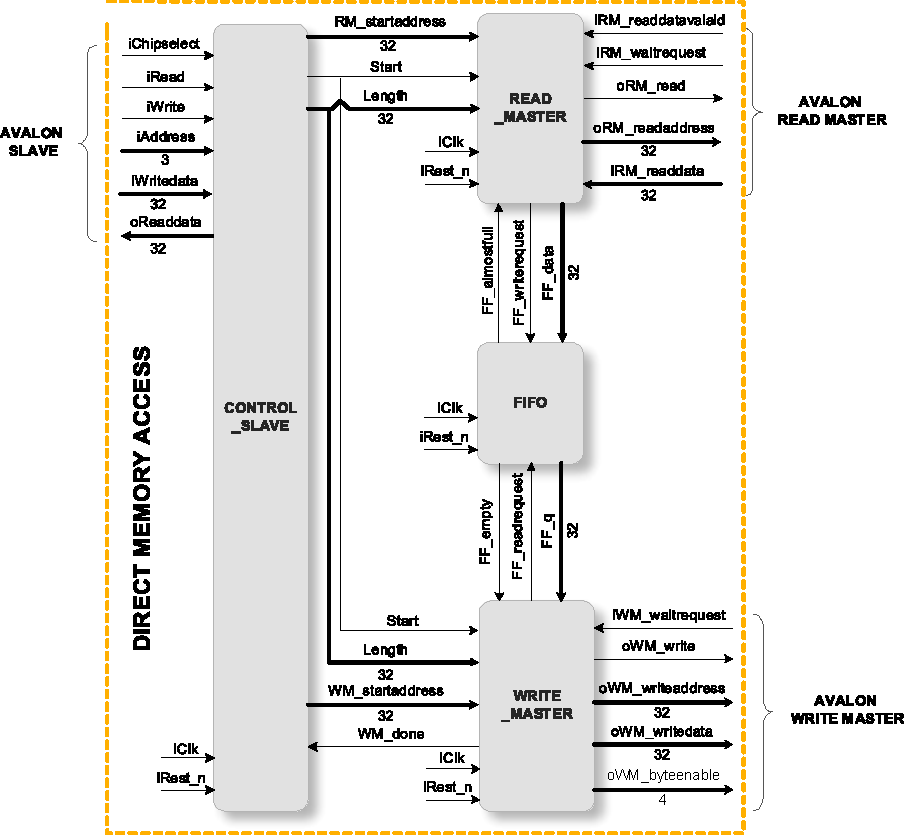
\includegraphics[width=\linewidth]{Images/02_09_DMABlockDiagram}
    \caption{Sơ đồ khối tổng thể của bộ điều khiển DMA.}
    \label{fig:02_09_DMA_BlockDiagram}
\end{figure}

\begin{figure}[htbp]
    \centering
    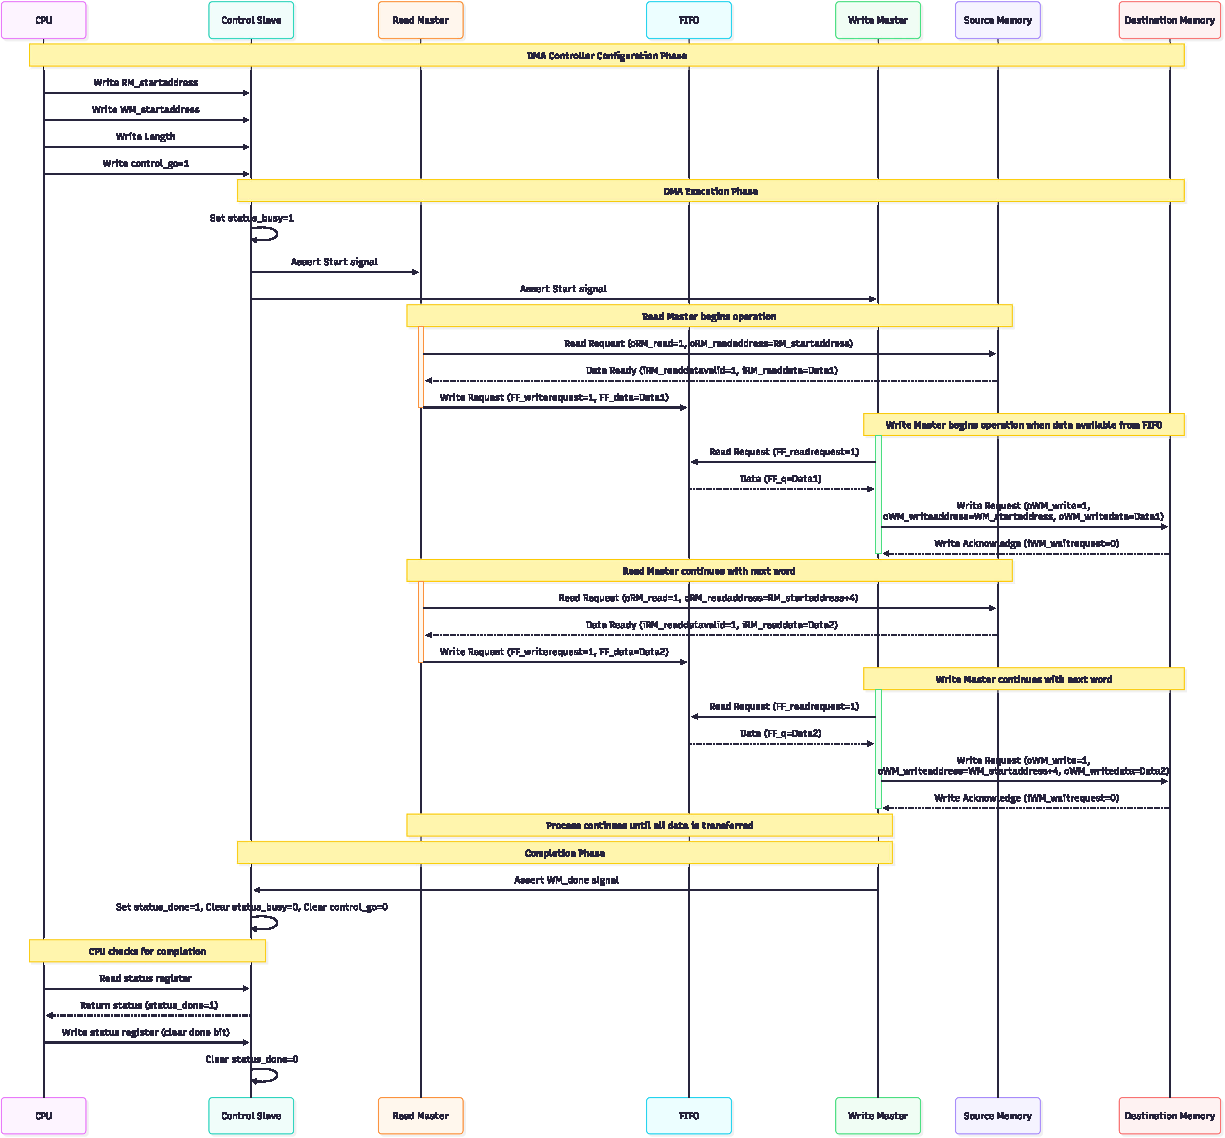
\includegraphics[width=\linewidth]{Images/02_10_SystemSequenceDiagram}
    \caption{Sơ đồ tuần tự hoạt động của DMA.}
    \label{fig:dma_flowchart_pdf}
\end{figure}

\begin{figure}[htbp]
    \centering
    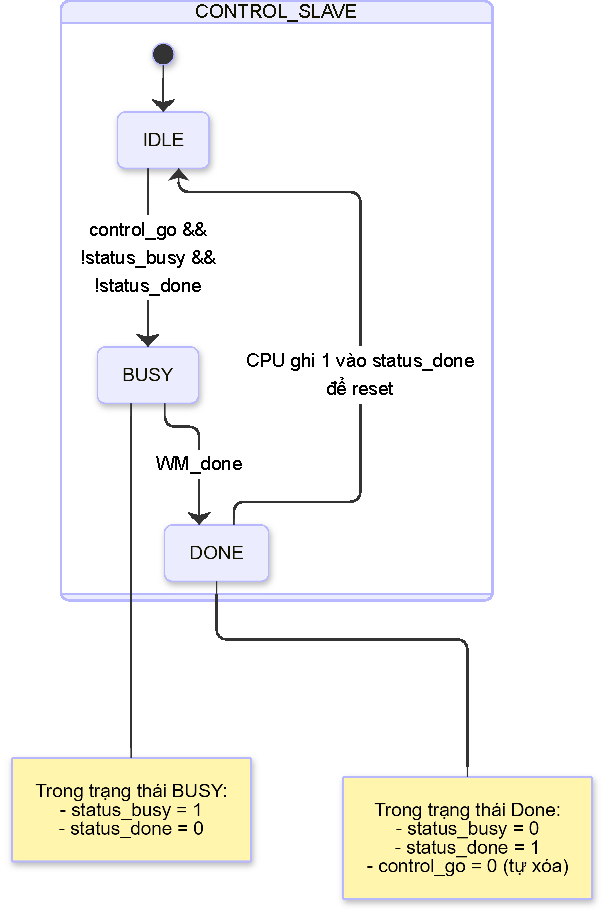
\includegraphics[width=0.5\linewidth]{Images/02_11_StateDiagram_ControlSlave}
    \caption{Sơ đồ trạng thái của module \texttt{CONTROL\_SLAVE}.}
    \label{fig:02_11_StateDiagram_ControlSlave}
\end{figure}

\begin{figure}[htbp]
    \centering
    % Subfigure for Memory Read
    \begin{subfigure}[b]{0.48\textwidth}
        \centering
        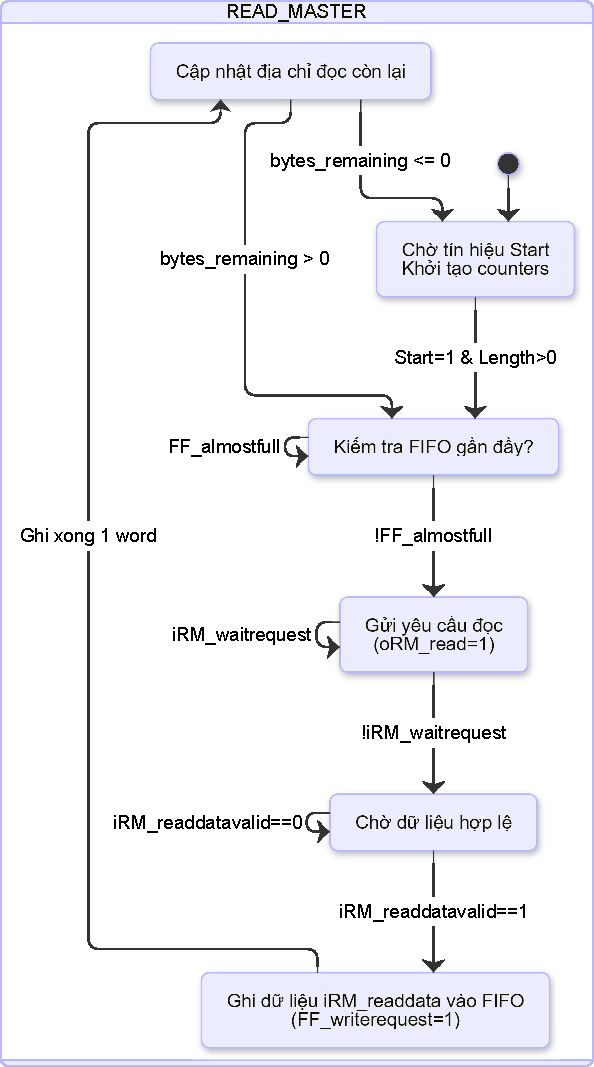
\includegraphics[width=\linewidth]{Images/02_12_StateDiagram_ReadMaster.pdf}
        \caption{\texttt{READ\_MASTER}.}
        \label{fig:02_12_StateDiagram_ReadMaster}
    \end{subfigure}
    \hfill % Thêm khoảng cách ngang
    % Subfigure for Memory Write
    \begin{subfigure}[b]{0.48\textwidth}
        \centering
        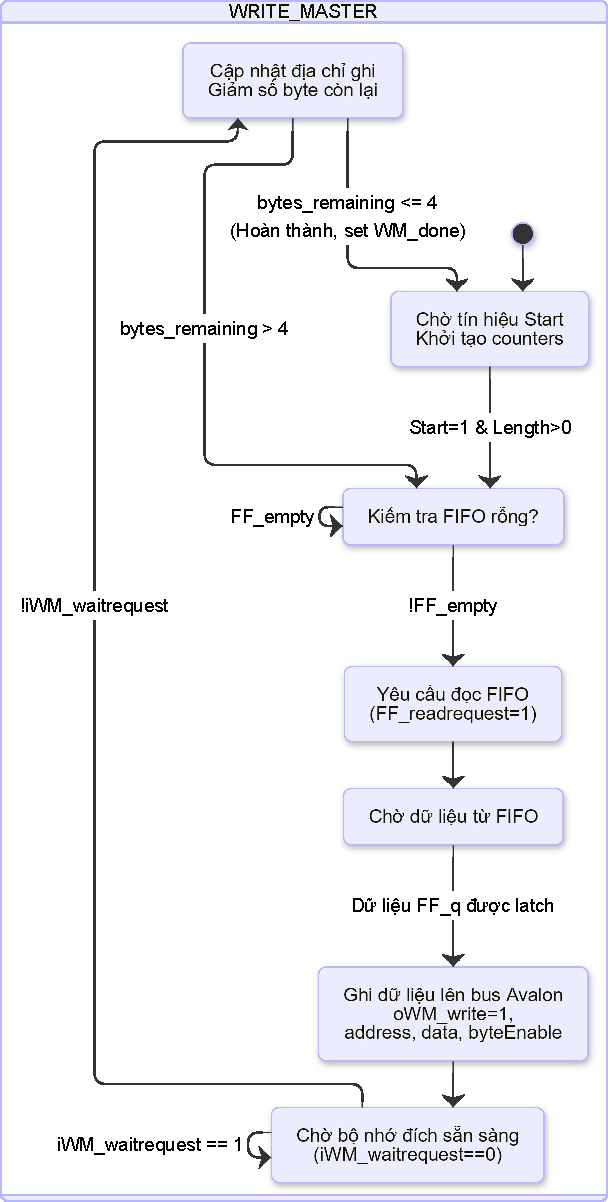
\includegraphics[width=\linewidth]{Images/02_13_StateDiagram_WriteMaster.pdf}
        \caption{\texttt{WRITE\_MASTER}.}
        \label{fig:02_13_StateDiagram_WriteMaster}
    \end{subfigure}
    \caption{Sơ đồ trạng thái các module.}
    \label{fig:memory_waveforms} % Nhãn chung cho cả cặp hình
\end{figure}

\subsection{Tín hiệu giao tiếp của DMA Controller} % Đã di chuyển bảng lên đây
Bảng \ref{tab:dma_signals} liệt kê các tín hiệu chính của module DMA Controller tùy chỉnh ở mức cao nhất (`DMAController.v`), thể hiện giao diện kết nối với CPU và hệ thống bus Avalon.

% --- Bảng tín hiệu DMA (Sử dụng định dạng gốc của người dùng) ---
\begin{table}[htbp]
    \centering
    \caption{Bảng mô tả tín hiệu chính của DMA Controller.}
    \label{tab:dma_signals}
    \begin{tabular}{@{}ccccp{7cm}@{}} % Định dạng gốc người dùng yêu cầu
        \toprule % Đường kẻ trên cùng
        \textbf{STT} & \textbf{Tên tín hiệu} & \textbf{Ngõ vào/ra} & \textbf{Số bit} & \textbf{Mô tả} \\
        \midrule % Đường kẻ giữa header và nội dung
        1 & \texttt{iClk} & In & 1 & Cấp xung clock 50 MHz cho DMA hoạt động \\
        2 & \texttt{iReset\_n} & In & 1 & \texttt{iReset\_n = 0}: reset lại DMA \\
        \midrule % Đường kẻ phân tách các nhóm tín hiệu
        \multicolumn{5}{@{}l}{\textbf{Giao tiếp Bus Avalon Slave (Từ CPU tới DMA)}} \\ % Sử dụng l căn trái cho tiêu đề nhóm
        \midrule
        3 & \texttt{iChipselect} & In & 1 & \texttt{iChipselect = 1}: cho phép truy xuất vào các thanh ghi trạng thái và điều khiển của DMA \\
        4 & \texttt{iRead} & In & 1 & \texttt{iRead = 1}: cho phép đọc giá trị của các thanh ghi trong DMA \\
        5 & \texttt{iWrite} & In & 1 & \texttt{iWrite = 1}: cho phép ghi giá trị vào các thanh ghi của DMA \\
        6 & \texttt{iAddress} & In & 3 & Chọn địa chỉ của thanh ghi cần đọc/ghi \\
        7 & \texttt{iWritedata} & In & 32 & Truyền giá trị cần ghi vào thanh ghi từ Avalon bus \\
        8 & \texttt{oReaddata} & Out & 32 & Xuất giá trị cần đọc từ thanh ghi ra Avalon bus \\
        \midrule
        \multicolumn{5}{@{}l}{\textbf{Giao tiếp Bus Avalon Read Master (Từ DMA tới Bộ nhớ Nguồn)}} \\
        \midrule
        9 & \texttt{iRM\_readdatavalid} & In & 1 & \texttt{=1}: báo hiệu \texttt{iRM\_readdata} hợp lệ \\
        10 & \texttt{iRM\_waitrequest} & In & 1 & \texttt{=1}: yêu cầu Read Master chờ \\
        11 & \texttt{oRM\_read} & Out & 1 & \texttt{=1}: yêu cầu đọc dữ liệu từ \texttt{oRM\_readaddress} \\
        12 & \texttt{oRM\_readaddress} & Out & 32 & Địa chỉ byte của vùng nhớ cần đọc \\
        13 & \texttt{iRM\_readdata} & In & 32 & Dữ liệu đọc được từ Avalon bus \\
        \midrule
        \multicolumn{5}{@{}l}{\textbf{Giao tiếp Bus Avalon Write Master (Từ DMA tới Bộ nhớ Đích)}} \\
        \midrule
        14 & \texttt{iWM\_waitrequest} & In & 1 & \texttt{=1}: yêu cầu Write Master chờ \\
        15 & \texttt{oWM\_write} & Out & 1 & \texttt{=1}: yêu cầu ghi dữ liệu vào \texttt{oWM\_writeaddress} \\
        16 & \texttt{oWM\_writeaddress} & Out & 32 & Địa chỉ byte của vùng nhớ cần ghi \\
        17 & \texttt{oWM\_writedata} & Out & 32 & Dữ liệu cần ghi ra Avalon bus \\
        18 & \texttt{oWM\_byteenable} & Out & 4 & Cho phép ghi từng byte (luôn là 4'b1111) \\
        \bottomrule
    \end{tabular}
\end{table}
% --- Kết thúc Bảng tín hiệu DMA ---

\FloatBarrier % Ngăn bảng và hình ảnh trôi qua section tiếp theo

\subsection{Hiện thực hóa Giao diện Avalon-MM trong DMA Controller}
Dựa trên đặc tả Avalon-MM, các giao diện của bộ điều khiển DMA tùy chỉnh được thiết kế như sau:
\begin{enumerate}
    \item \textbf{Giao diện Slave của \texttt{CONTROL\_SLAVE}:} Module này hoạt động như một Slave đơn giản, không sử dụng \texttt{waitrequest}. Nó giải mã \texttt{iAddress} khi \texttt{iChipselect=1} để đọc/ghi các thanh ghi nội bộ.
        \begin{itemize}
            \item \textbf{Khi đọc (\texttt{iRead=1}):} Dữ liệu từ thanh ghi tương ứng (địa chỉ nguồn/đích, độ dài, control, status) được đưa ra \texttt{oReaddata}. Hình \ref{fig:02_03_avalon_slave_read_sub}.
            \item \textbf{Khi ghi (\texttt{iWrite=1}):} Dữ liệu \texttt{iWritedata} được ghi vào thanh ghi cấu hình (địa chỉ nguồn/đích, độ dài) hoặc bit GO của thanh ghi điều khiển. Ghi 1 vào bit 0 của thanh ghi trạng thái sẽ xóa cờ Done. Hình \ref{fig:02_04_avalon_slave_write_sub}.
        \end{itemize}

    % Figures 02_03 and 02_04 side-by-side
    \begin{figure}[htbp]
        \centering
        \begin{subfigure}[b]{0.48\textwidth}
            \centering
            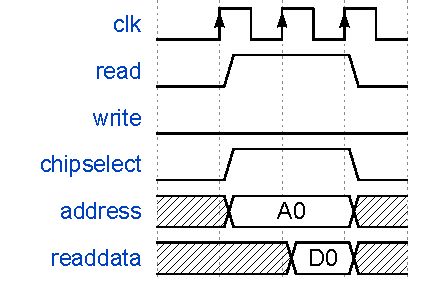
\includegraphics[width=\linewidth]{Images/02_03_AvalonSlave_ReadWaveform.pdf}
            \caption{Giản đồ sóng đọc Slave.}
            \label{fig:02_03_avalon_slave_read_sub}
        \end{subfigure}
        \hfill
        \begin{subfigure}[b]{0.48\textwidth}
            \centering
            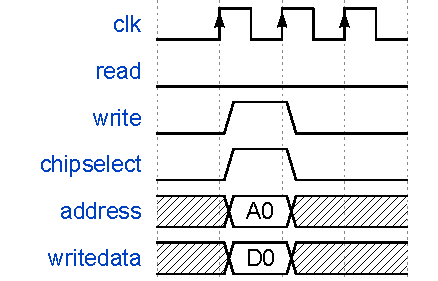
\includegraphics[width=\linewidth]{Images/02_04_AvalonSlave_WriteWaveform.pdf}
            \caption{Giản đồ sóng ghi Slave.}
            \label{fig:02_04_avalon_slave_write_sub}
        \end{subfigure}
        \caption{Giản đồ sóng đọc và ghi của giao tiếp Avalon-MM Slave.}
        \label{fig:avalon_slave_waveforms}
    \end{figure}

    \item \textbf{Giao diện Master của \texttt{READ\_MASTER}:} Module chủ động tạo giao dịch đọc, xử lý \texttt{waitrequest} và \texttt{readdatavalid}.
        \begin{itemize}
            \item Kích hoạt \texttt{oRM\_read=1} và đưa ra \texttt{oRM\_readaddress}.
            \item Nếu \texttt{iRM\_waitrequest=1}, giữ nguyên tín hiệu và trạng thái.
            \item Khi \texttt{iRM\_waitrequest=0}, chờ \texttt{iRM\_readdatavalid=1} mới lấy dữ liệu \texttt{iRM\_readdata} và ghi vào FIFO. Hình \ref{fig:02_05_avalon_master_read}.
        \end{itemize}

    \begin{figure}[htbp]
        \centering
        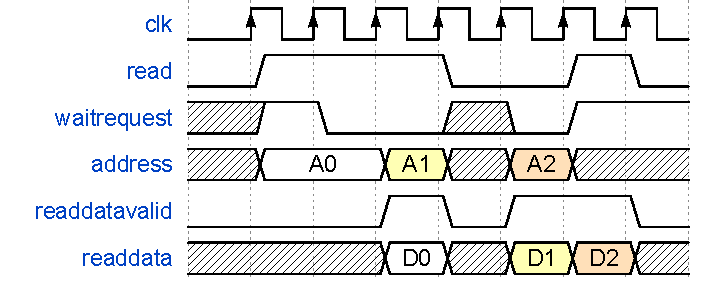
\includegraphics[width=\linewidth]{Images/02_05_AvalonMaster_ReadWaveform.pdf}
        \caption{Giản đồ sóng đọc của giao tiếp Avalon-MM Master.}
        \label{fig:02_05_avalon_master_read}
    \end{figure}

    \item \textbf{Giao diện Master của \texttt{WRITE\_MASTER}:} Module chủ động tạo giao dịch ghi, xử lý \texttt{waitrequest}.
        \begin{itemize}
            \item Kích hoạt \texttt{oWM\_write=1}, đưa ra \texttt{oWM\_writeaddress}, \texttt{oWM\_writedata}, và \texttt{oWM\_byteenable = 4'b1111}.
            \item Nếu \texttt{iWM\_waitrequest=1}, giữ nguyên tất cả tín hiệu đầu ra và trạng thái.
            \item Khi \texttt{iWM\_waitrequest=0}, giao dịch ghi được xem là hoàn thành, FSM chuyển trạng thái. Hình: \ref{fig:02_06_avalon_master_write}.
        \end{itemize}

    \begin{figure}[htbp]
        \centering
        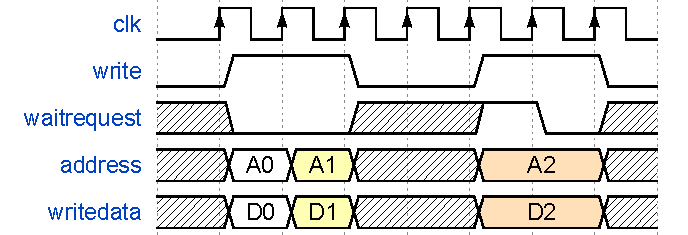
\includegraphics[width=\linewidth]{Images/02_06_AvalonMaster_WriteWaveform.pdf}
        \caption{Giản đồ sóng ghi của giao tiếp Avalon-MM Master.}
        \label{fig:02_06_avalon_master_write}
    \end{figure}
\end{enumerate}
Việc thiết kế các giao diện DMA dựa trên và tuân thủ chặt chẽ đặc tả Avalon-MM là yếu tố then chốt đảm bảo bộ điều khiển DMA tùy chỉnh có thể hoạt động chính xác và tích hợp liền mạch vào hệ thống SoC Nios V trên Platform Designer.

\begin{figure}[htbp]
    \centerin
    % Subfigure for Memory Read
    \begin{subfigure}[b]{0.48\textwidth}
        \centering
        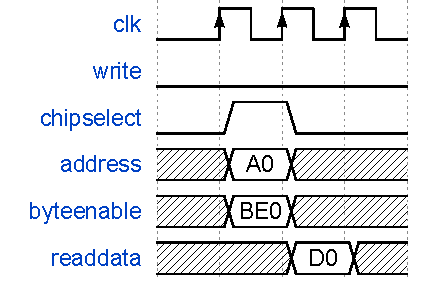
\includegraphics[width=\linewidth]{Images/02_07_Memory_ReadWaveform.pdf}
        \caption{Giản đồ sóng đọc Memory.}
        \label{fig:02_07_memory_read_sub}
    \end{subfigure}
    \hfill
    \begin{subfigure}[b]{0.48\textwidth}
        \centering
        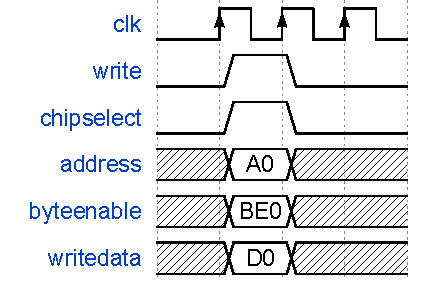
\includegraphics[width=\linewidth]{Images/02_08_Memory_WriteWaveform.pdf}
        \caption{Giản đồ sóng ghi Memory.}
        \label{fig:02_08_memory_write_sub}
    \end{subfigure}
    \caption{Giản đồ sóng đọc và ghi bộ nhớ qua giao tiếp Avalon-MM.}
    \label{fig:memory_waveforms}
\end{figure}
